\section{System overview}
%%%%%%%%%%%% MID WAY AGENDA %%%%%%%%%%%%%%
\begin{frame}<beamer>
\frametitle{System overview}
\begin{figure}
	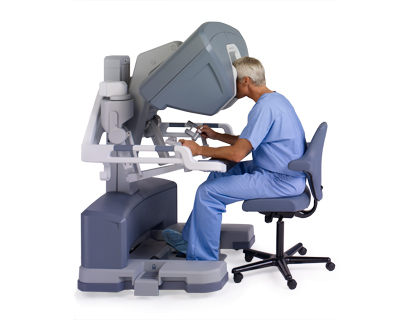
\includegraphics[width=0.2\textwidth]{Billeder/Dan/console.jpg}
	\hspace{16.3 mm} $\Rightarrow $
	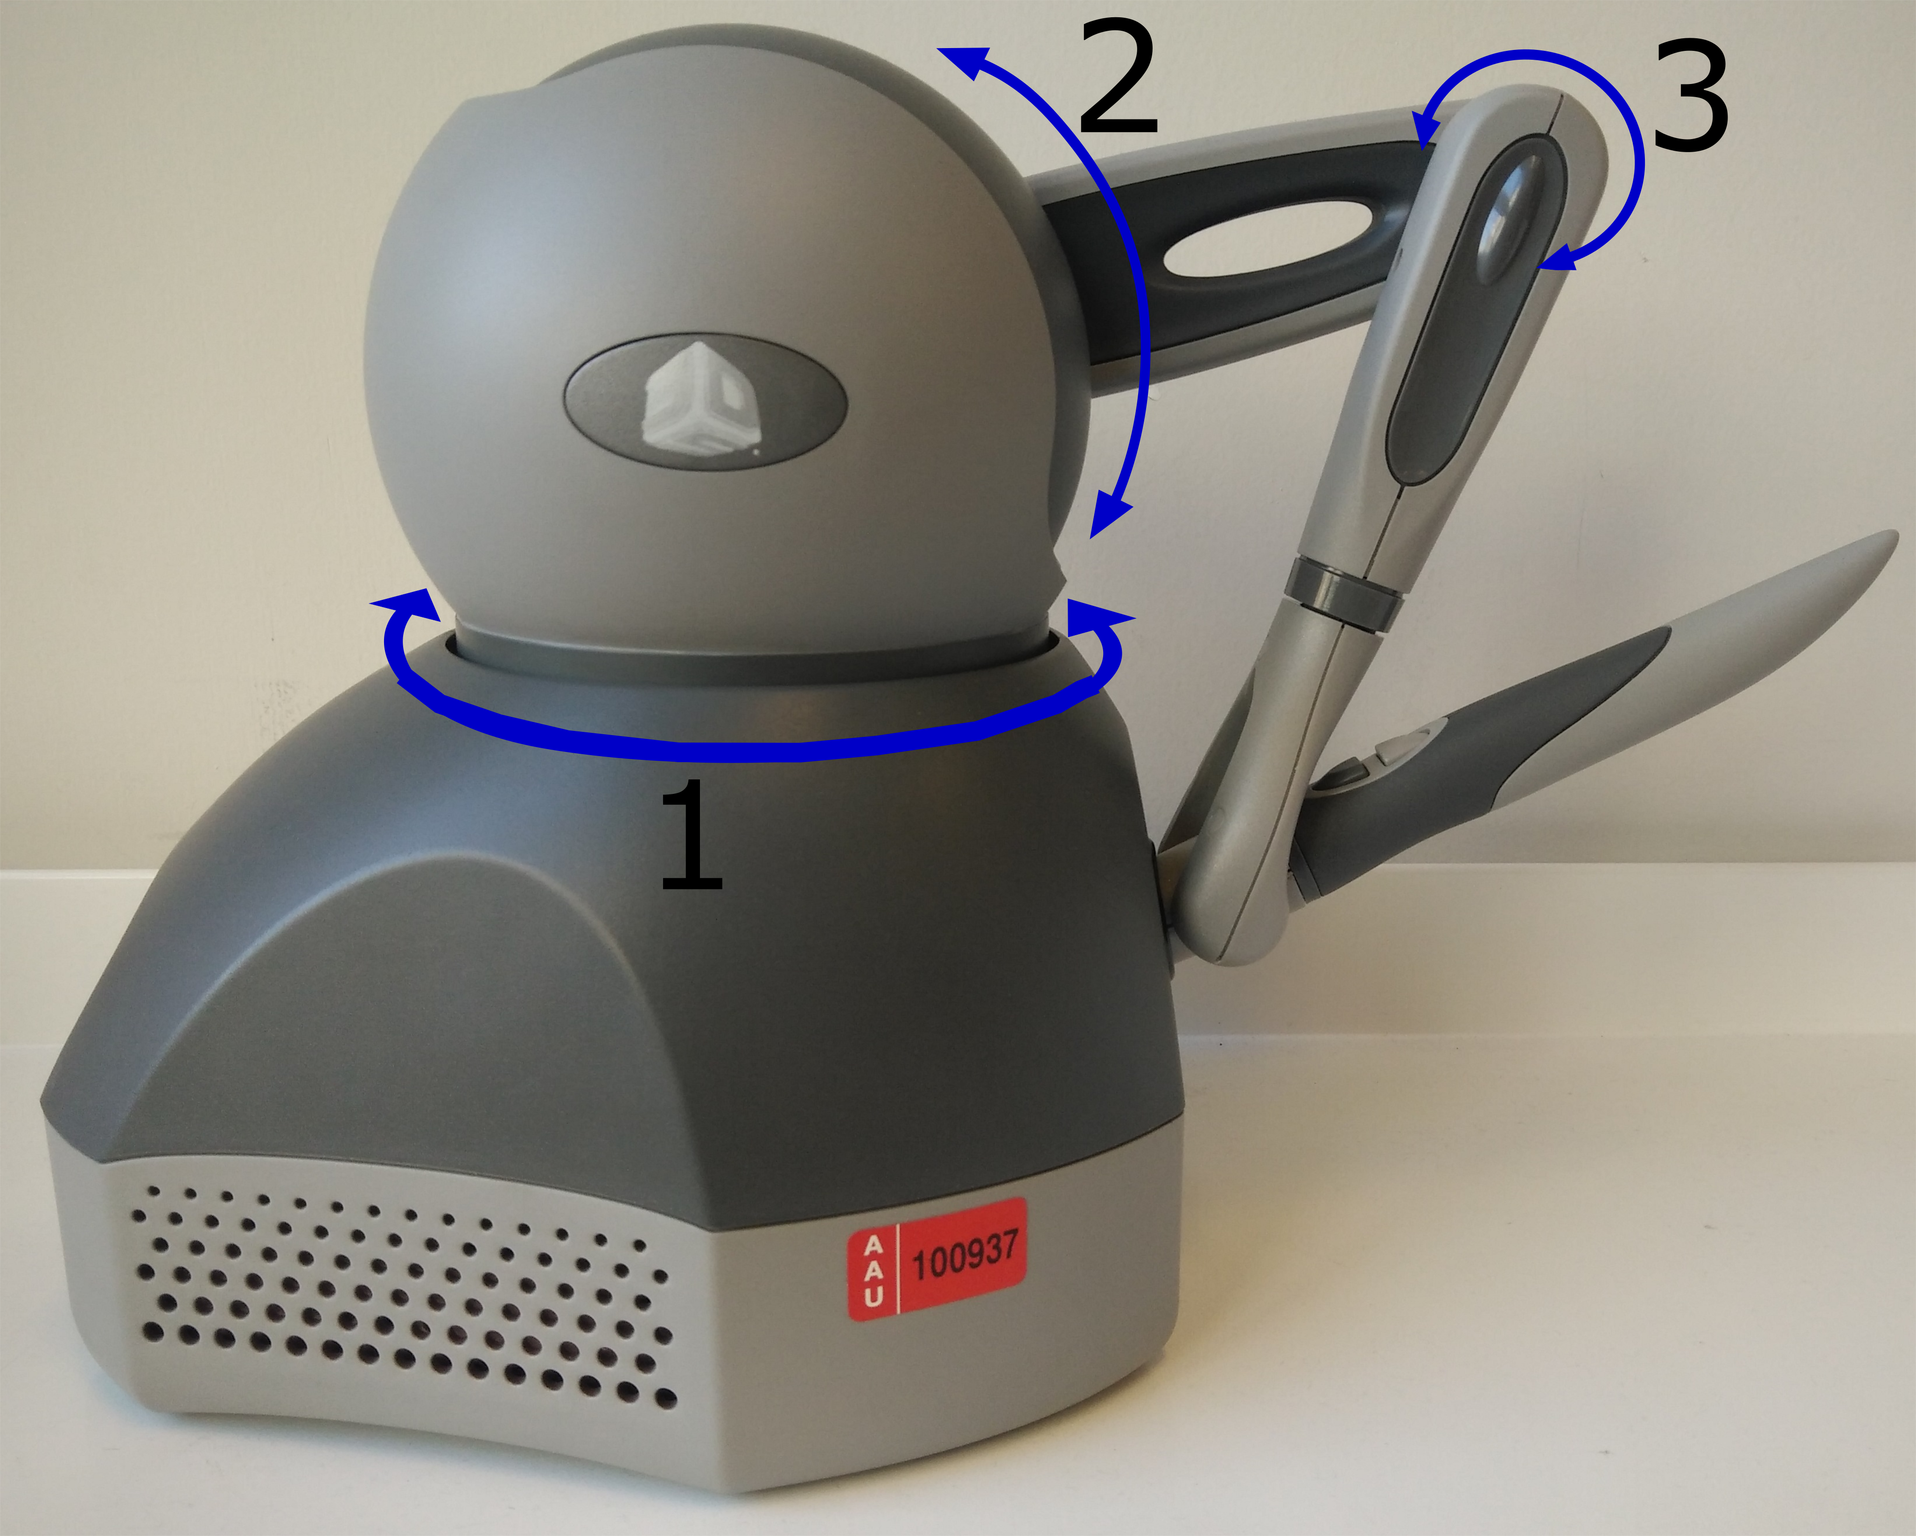
\includegraphics[width=0.2\textwidth]{Billeder/Dan/gt.png}
\end{figure}

\resizebox{\textwidth}{!}{
	\begin{tikzpicture}
	
	
	\node[box] (Opt) at (0,0) {Operator};
	\node[box] (Geo) at ($(3,0) + (Opt)$) {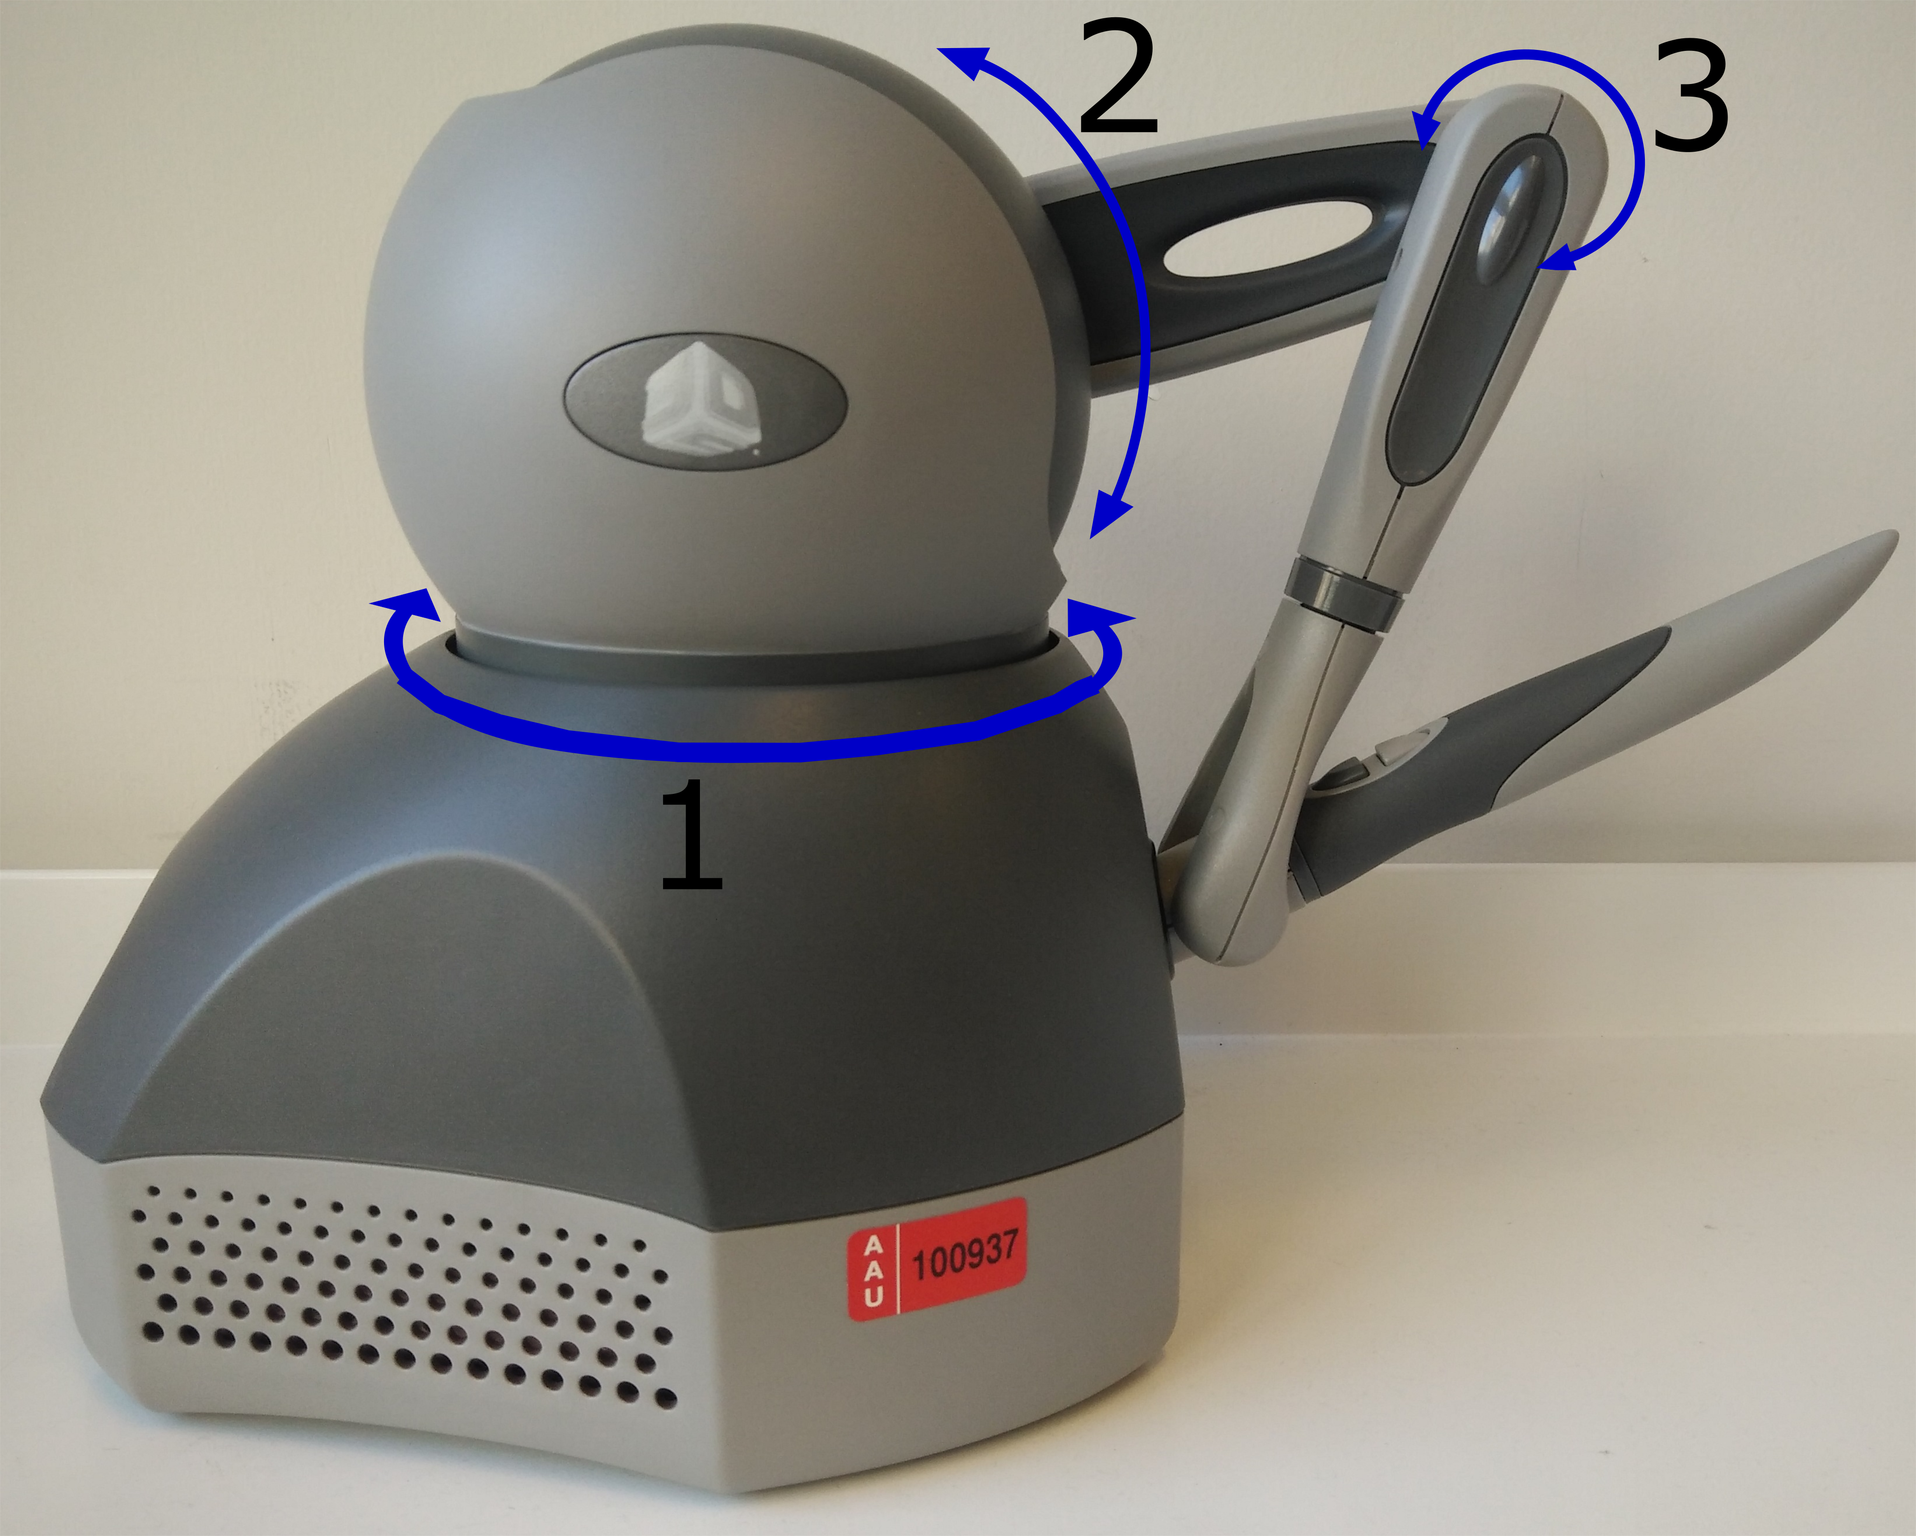
\includegraphics[width=0.2\textwidth]{Billeder/Dan/gt.png}};
	\node[box] (ros) at ($(3,0) + (Geo)$) {Computer};
	\node[box] (davin) at ($(3,0) + (ros)$) {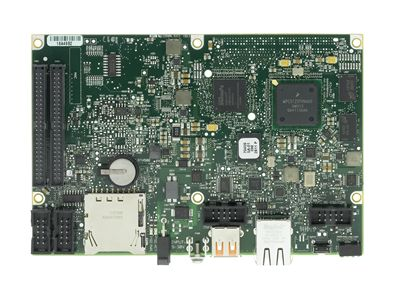
\includegraphics[width=0.2\textwidth]{Billeder/Dan/sbRIO9636.png}};
	\node[box] (end) at ($(3,0) + (davin)$) {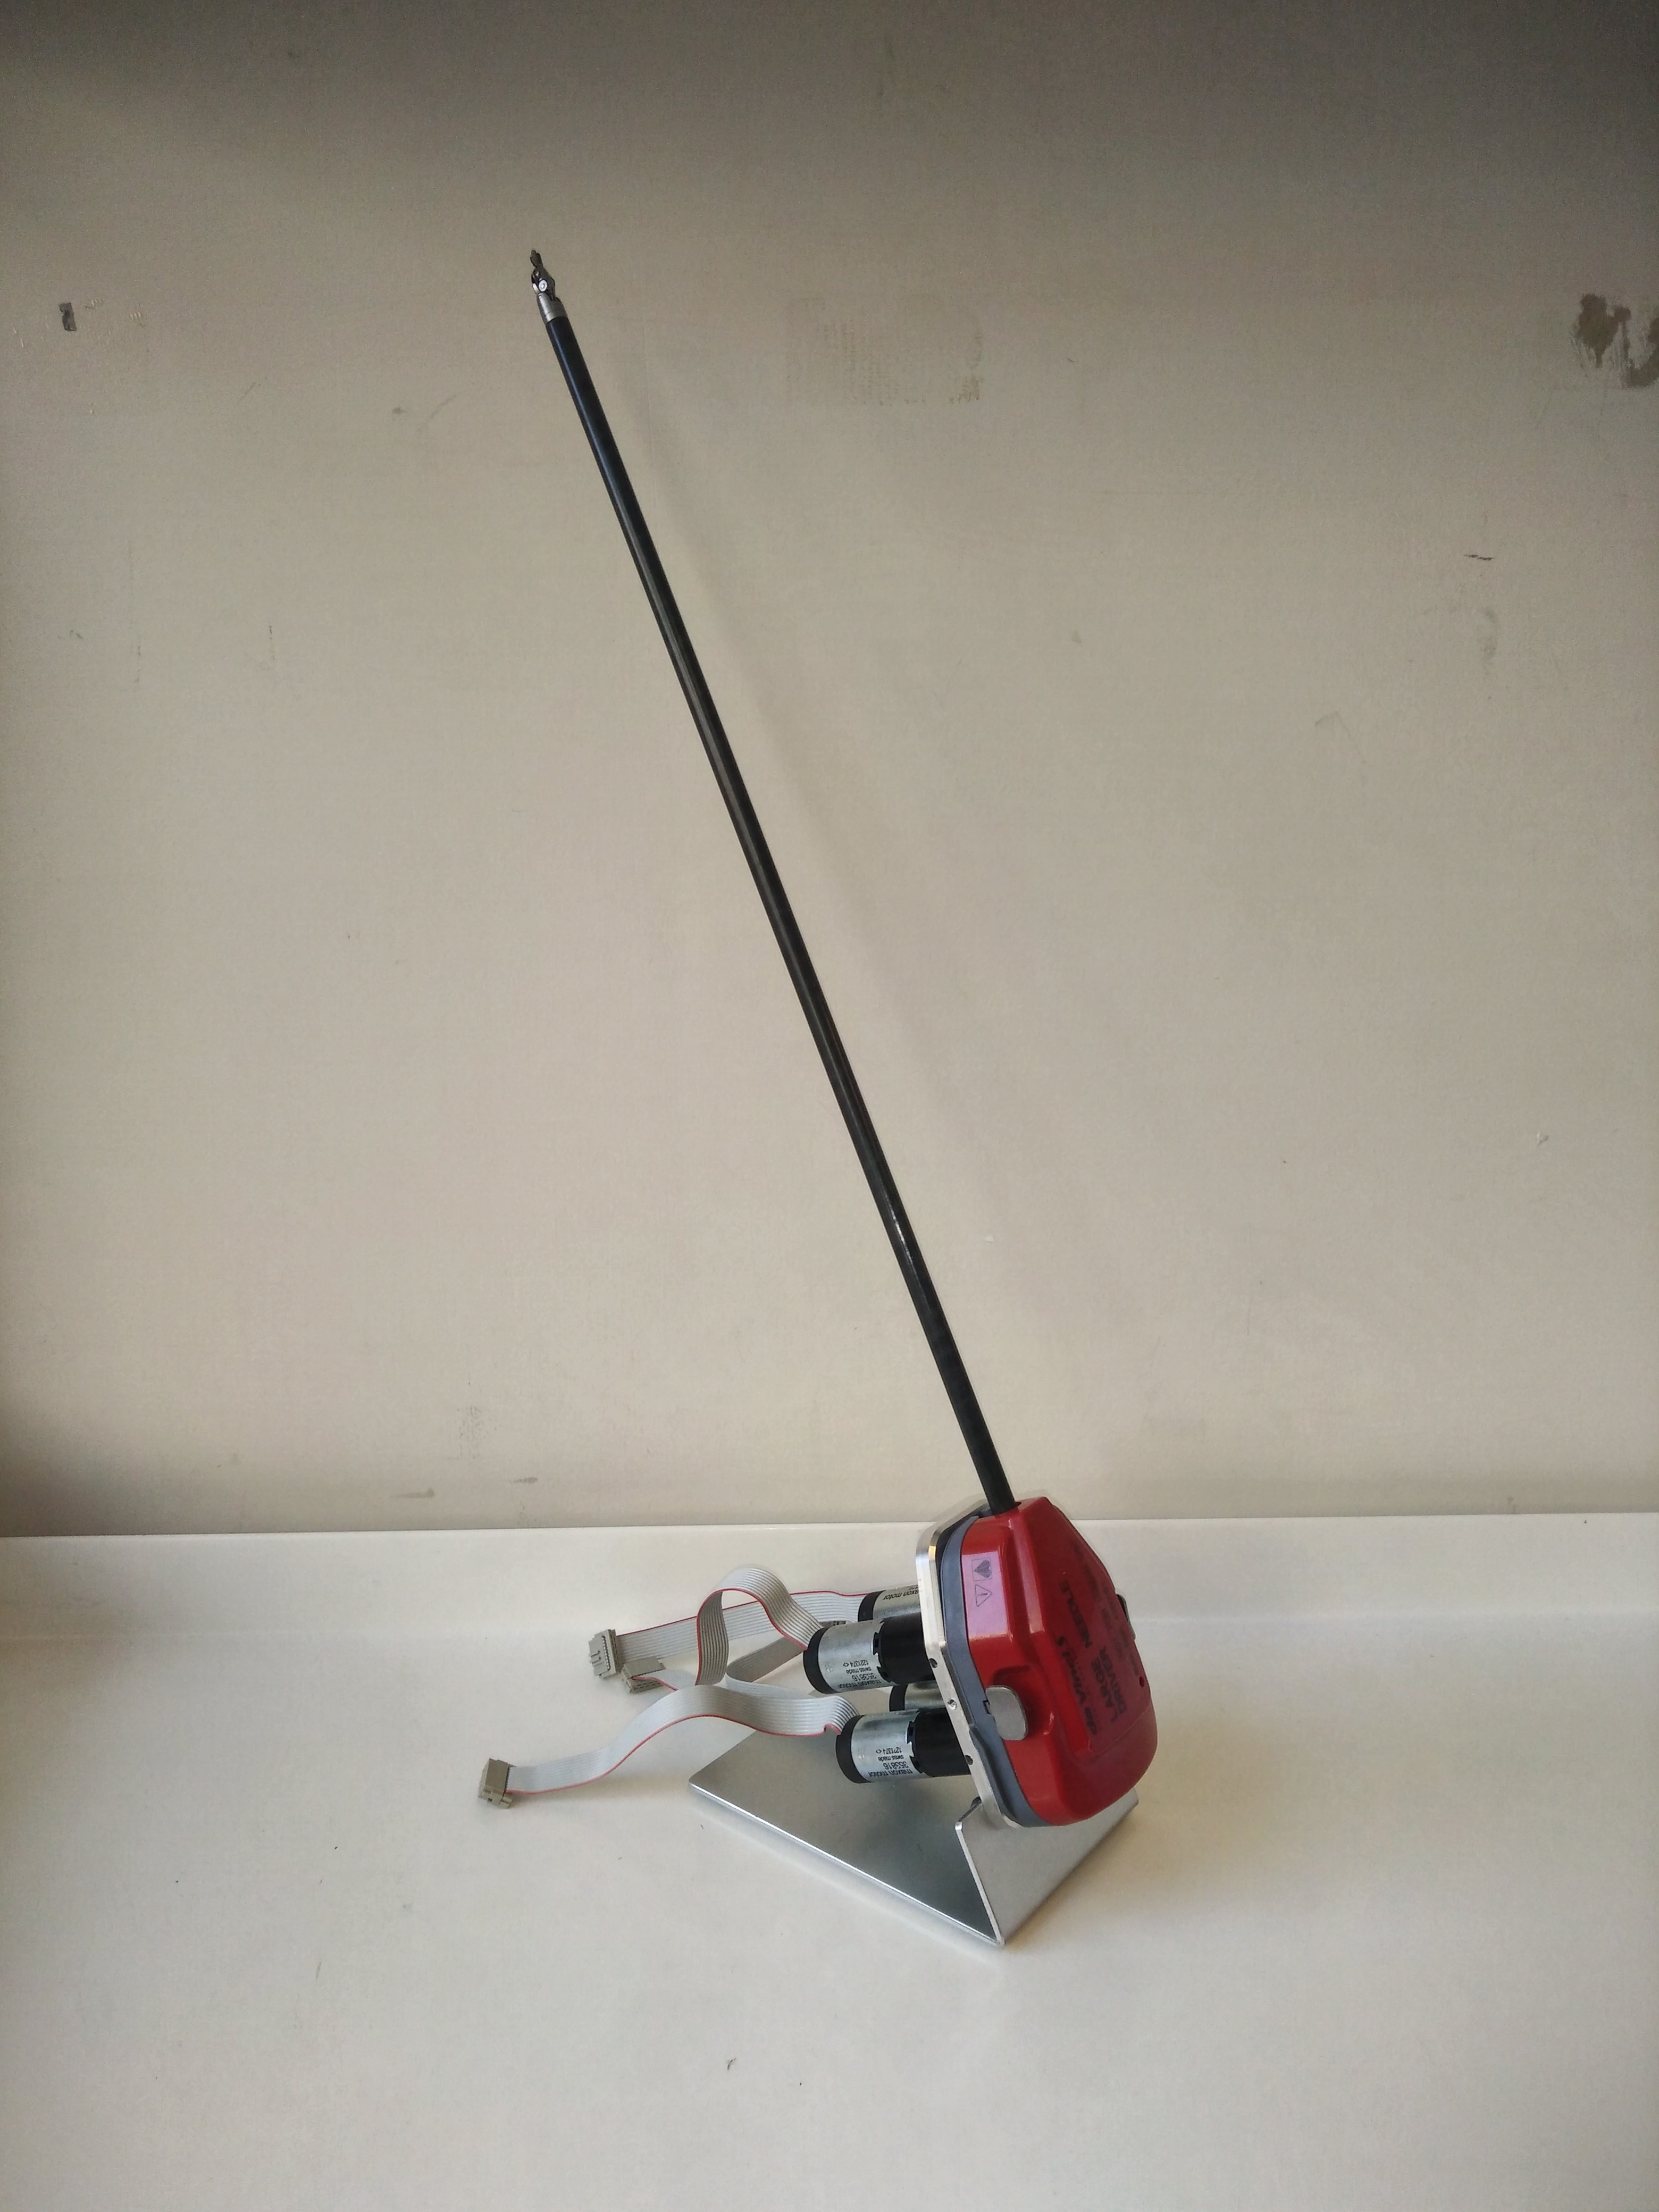
\includegraphics[width=0.2\textwidth]{Billeder/Dan/endowrist.jpg}};
	
	
	\draw[->, ultra thick] ([yshift=0.3cm]Opt.east) -- ([yshift=0.3cm]Geo.west);
	\draw[->, ultra thick] ([yshift=0.3cm]Geo.east) -- ([yshift=0.3cm]ros.west);
	\draw[->, ultra thick] ([yshift=0.3cm]ros.east) -- ([yshift=0.3cm]davin.west);
	\draw[->, ultra thick] ([yshift=0.3cm]davin.east) -- ([yshift=0.3cm]end.west);
	
	
	\draw[<-, ultra thick] ([yshift=-0.3cm]Opt.east) -- ([yshift=-0.3cm]Geo.west);
	\draw[<-, ultra thick] ([yshift=-0.3cm]Geo.east) -- ([yshift=-0.3cm]ros.west);
	\draw[<-, ultra thick] ([yshift=-0.3cm]ros.east) -- ([yshift=-0.3cm]davin.west);
	%\draw[<-, ultra thick] ([yshift=-0.3cm]davin.east) -- ([yshift=-0.3cm]end.west);
	
	\node at (1.5,1) {Position};
	\node at (4.5,1) {Position};
	% \node at (7.5,1) {yes};
	% \node at (10.5,1) {yes};
	
	\node at (1.5,-1) {Force};
	\node at (4.5,-1) {Force};
	\node at (10.5,1) {Torque};
	% \node at (10.5,1) {yes};
	%\node at (7.5,1.5) {Motor enable};
	\node at (7.5,1) {Position};
	\node at (7.5,-1) {Position};
	\node at (7.5,-1.5) {Velocity};
	\node at (7.5,-2) {Current};
	
	\end{tikzpicture}
}
\end{frame}